\documentclass[logo,reportComp]{thesis}
\usepackage[python,pseudo,linenum]{mypackage}
\hypersetup{colorlinks=false,urlbordercolor=red}
\usepackage{relsize}

\setcounter{secnumdepth}{4}
\titleformat{\paragraph}{\bfseries}{\alph{paragraph})~~}{0em}{}
\titlespacing*{\paragraph}{0pt}{0pt}{0pt}[0pt]

\title{人工神经网络}
\subtitle{Lab 3:全连接神经网络(FCN)}
\school{数据科学与计算机学院}
\author{陈鸿峥}
\classname{17大数据与人工智能}
\stunum{17341015}
\headercontext{人工神经网络作业}

\let\emph\relax % there's no \RedeclareTextFontCommand
\DeclareTextFontCommand{\emph}{\kaiti\em}
\AtBeginEnvironment{quote}{\kaiti\small}

\begin{document}

\maketitle
\tableofcontents

\newpage

\section{框架概览}
虽然本次作业只是让我们实现一个3层的全连接神经网络,不过为了更加深入理解神经网络框架的原理,在本次实验中我借鉴了PyTorch的API接口,尝试用更好的模块化方式实现一个\textbf{简易版的神经网络框架}。
由于基础设施(老师提供的模板)是基于PyTorch的,因此我的框架也是基于PyTorch的Tensor类进行封装,命名为TinyTorch。

TinyTorch的整体架构如图\ref{fig:overview}所示,主要分为网络层(Layer)、模块(Module)、损失函数(Loss)、优化器(Optimizer)四个部分。
数据通过前端读入后,经过神经网络模块前向传播(forward),计算损失及其梯度,并反向传播(backward),输出结果。
\begin{figure}[H]
\centering
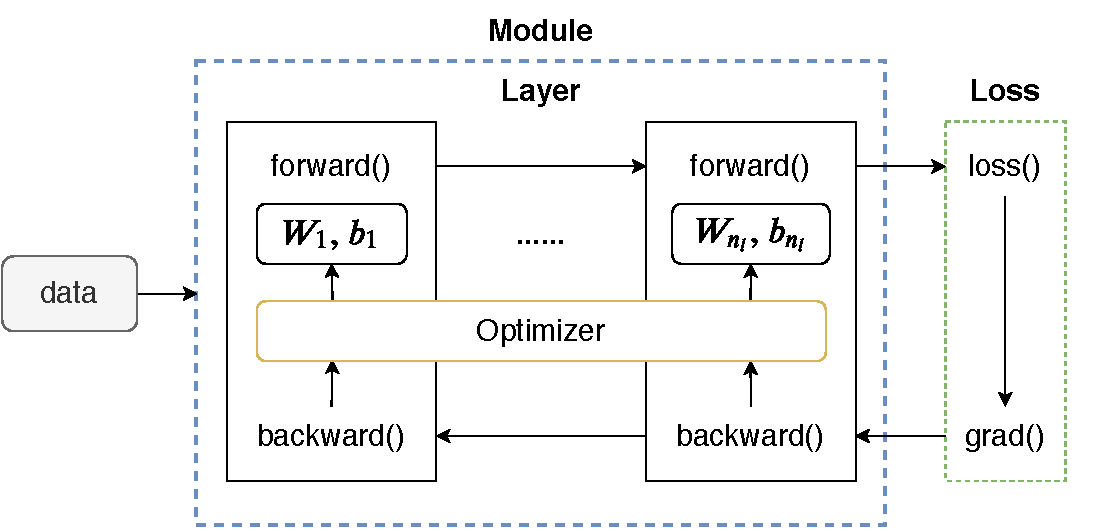
\includegraphics[width=0.7\linewidth]{fig/tinytorch.pdf}
\caption{TinyTorch概览}
\label{fig:overview}
\end{figure}

各模块功能如下:
\begin{itemize}
	\item 网络层:包含神经网络层(如线性层和卷积层)和激活函数层。
	\item 模块:将网络层打包封装起来的完整神经网络,继承自基类\verb'nn.Module',用户可自定义传播方式。
	\item 损失函数:计算损失函数及其梯度。
	\item 优化器:用于更新网络层参数。
\end{itemize}

下面会详细介绍各个模块的实现方式。

\section{模块实现}
为打包成可在Python中调用的库,需要在顶层文件夹添加\verb'__init__.py'文件,内容为空即可。

\subsection{网络层}
在\verb'tinytorch/nn.py'中实现,首先实现基类\verb'Layer',内容如下。
作为网络层的抽象,其需要有前向传播和后向传播功能,故分别实现了\verb'forward'和\verb'backward'两个函数。
在前向传播中需要将上一层的输出(也即当前层的输入)先保存起来,方便反向传播进行计算。
而具体前后向传播怎么算,则由子类进行定义。
同时,为了方便像PyTorch中一样用括号形式直接调用,这里重载了\verb'__call__'函数。
\lstinputlisting[linerange={4-28},firstnumber=4]{../tinytorch/nn.py}

有了基类便可实现线性层\verb'Linear',其前向传播计算方式如下
\[\layer{\vz}{l}=\mathrm{Linear}(\layer{\va}{l-1}) = \layer{\va}{l-1} W + \vb\]
其中$W\in\rr^{d_in\times d_out}$为权重参数,$\vb\in\rr^{1\times d_out}$为偏置参数,$\layer{\va}{k-1}$为上一层激活后的输出。
注意这里将权重参数右乘输入向量,只是为了方便存储和计算,与后面的推导可能存在差异。

反向传播(具体理论推导见第\ref{sec:theory}节)
\[\begin{cases}
\pd{\mL}{W}=\layer{\va}{l-1}^\T\layer{\delta}{l}\\
\pd{\mL}{\vb}=\layer{\delta}{l}
\end{cases}\]
同时一并计算$\layer{\tilde{\delta}}{l-1}=\layer{\delta}{l}W^\T$。
另外注意由于是批训练,故$\partial\mL/\partial \vb$计算时是对批内所有值求和。

初始化$W$和$\vb$直接调用\verb'torch.nn.init.kaiming_uniform_',存储在\verb'params'字典中。
同时,开设两个元素\verb'd_w'和\verb'd_b'存储梯度。

进而可重载前向和后向传播函数,并得到完整线性层实施如下。
\lstinputlisting[linerange={46-82},firstnumber=46]{../tinytorch/nn.py}

\subsection{激活函数}
激活函数的基类\verb'Activation'实现在\verb'tinytorch/nn.py'中,作为特殊的网络层,依然从\verb'Layer'继承得到。
由于激活函数层反向传播的模式是固定的,
\[\layer{\delta}{l}=\layer{\tilde{\delta}}{l}\odot h'(\layer{\vz}{l})\]
故可以再做一层抽象,新增的激活函数只需重载导函数$h'(\cdot)$即可。
基类定义如下。
\lstinputlisting[linerange={29-44},firstnumber=29]{../tinytorch/nn.py}

其他激活函数可参见\verb'tinytorch/activation.py'。
由于这一部分就是将激活函数用向量形式表示,并求出其导函数,故在此不再赘述。
这里关注Sigmoid和Tanh的导函数
\[\begin{aligned}
\sigma'(\vx)&=\sigma(\vx)(1-\sigma(\vx))\\
\tanh'(\vz)&=1-\tanh^2(\vx)
\end{aligned}\]
完整代码实现如下。
\lstinputlisting[linerange={5-46},firstnumber=5]{../tinytorch/activation.py}

\subsection{模块}
模块基类\verb'Module'定义在\verb'tinytorch/nn.py'中,为了最大程度减少用户的代码编写量,因此这里将反向传播部分也实现在\verb'backward'中,但由于没有用重载运算符的方式实现自动微分(automatic differentiation, AD)功能\footnote{这需要自己定义Tensor类,并对运算符进行重载,但由于老师的框架直接调用PyTorch的DataLoader,已经将数据打包成了PyTorch自带的Tensor类,因此没有办法重新进行封装。},故还是需要用户将计算出来的损失函数的梯度值输入,然后调用\verb'backward'函数进行反向传播。
同时,在初始化阶段,也需要用户调用\verb'add_layers'函数,将网络层\textbf{依序}添加到列表中。
这样回传时就可以直接逆向遍历网络层,逐一调用网络层的\verb'backward'实现反向传播。
代码如下。
\lstinputlisting[linerange={84-110},firstnumber=84]{../tinytorch/nn.py}

\subsection{损失函数}
损失函数定义在\verb'tinytorch/loss.py'中,同样有基类\verb'Loss'。
派生类需要重载前向计算的\verb'loss'函数,以及反向传播的\verb'grad'函数。
这一部分还是因为没有实现AD,故没有办法像PyTorch一样做到\verb'loss.backward()'回传,只能分开实现计算梯度后再回传。

下面以交叉熵函数为例,前向传播公式为(已经结合了Softmax和NLLLoss)
\begin{equation}
\label{equ:cross_entropy}
\mL=\frac{1}{N}\sum_{i=1}^N\mathrm{Loss}(\smp{\vx}{i},\smp{y}{i})
=-\frac{1}{N}\sum_{i=1}^N\log\frac{\exp(\smp{\vx}{i}[\smp{y}{i}])}{\sum_{j=1}^d\exp(\smp{\vx}{i}_j)}
=-\frac{1}{N}\sum_{i=1}^N\lrp{\smp{\vx}{i}[\smp{y}{i}]-\log\lrp{\sum_{j=1}^d\exp(\smp{\vx}{i}_j)}}
\end{equation}
这一部分要特别小心,非常容易出错。
在具体实施上需要关注以下两个点:
\begin{itemize}
	\item \textbf{避免指数爆炸}:直接计算Softmax会导致指数过大,因此需要对分子分母同除$\exp(\max)$,相当于指数作差,确保指数都小于等于$0$,进而指数项落在$(0,1]$的区间
	\item \textbf{避免对数爆炸}:由于计算机精度原因,一些过小的值会被直接当作$0$处理(数值下溢),若直接取对数会导致出现\verb'-inf',故应该把Softmax计算和NLLLoss计算合并,变成(\ref{equ:cross_entropy})后面的公式,对指数项求和后可确保值不再为$0$,进而可以正常取对数。
\end{itemize}

反向传播的公式为(推导见第\ref{sec:theory}节)
\[\layer{\tilde{\delta}}{n_l}=\layer{\va}{n_l}-\vy\]
最终代码实现如下。
\lstinputlisting[linerange={14-46},firstnumber=14]{../tinytorch/loss.py}

\subsection{优化器}
优化器定义在\verb'tinytorch/optim.py'中,基类\verb'Optimizer'给出梯度归零的初始化方法\verb'zero_grad',需要在每轮迭代开始前调用。

带动量的SGD更新公式如下。
\[\begin{cases}
    \vnu_{t+1}=\textcolor{red}{\gamma\vnu_t}-\eta\nabla\mL(\vtheta_t)\\
    \vtheta_{t+1}=\vtheta_t+\vnu_{t+1}
\end{cases}\]
注意需要为每个参数单独创建$\vnu$值,且初始化为$\vzero$。
\lstinputlisting[linerange={3-45},firstnumber=3]{../tinytorch/optim.py}

\section{全连接网络搭建}
虽然在TinyTorch中调用了PyTorch中一些基本计算函数,如\verb'sum'、\verb'max'等,但其实可以全部换成NumPy实现,因为PyTorch与TinyTorch并不是紧耦合关系。

三层神经网络定义在\verb'fcn.py'中,全部采用全连接层,中间激活函数用ReLU,维度变换如下
\[INPUT(784)\to FC(256)\to FC(128)\to FC(10)\]
\lstinputlisting[linerange={33-53},firstnumber=33]{../fcn.py}

采用交叉熵损失函数及带冲量的SGD进行优化。
具体训练使用接口基本与PyTorch一致,唯一不同是在反向传播部分,TinyTorch需要用下面的方式进行调用。
\lstinputlisting[linerange={160-160},firstnumber=160]{../fcn.py}
其他部分按照老师所给的框架直接执行即可。

\section{实验设置}
实验MNIST数据集上进行测试,并将TinyTorch与PyTorch进行比较。
完整代码可见\verb'fcn.py'和\verb'fcn_torch.py',后者是PyTorch实现的神经网络,采用的网络结构、优化器及损失函数均与TinyTorch相同。

实验在CPU上进行,超参数设置如表\ref{tab:hyper}所示。
\begin{table}[H]
\centering
\caption{超参数}
\label{tab:hyper}
\begin{tabular}{|c|c|c|}\hline
学习率 & \verb'lr' & 0.02 \\\hline
动量 & \verb'momentum' & 0.9 \\\hline
批量大小 & \verb'batch_size' & 128 \\\hline
迭代次数 & \verb'epoch' & 20 \\\hline
\end{tabular}
\end{table}

\section{实验结果}
实验结果如图\ref{fig:acc}所示,TinyTorch与PyTorch在测试集的精度最终都达到100\%,而测试集精度都达到96\%以上,可见TinyTorch已经非常接近PyTorch的水平,而存在的一些差异则是在网络层的初始化、权重衰减、以及优化器的实现上面。
\begin{figure}[H]
\centering
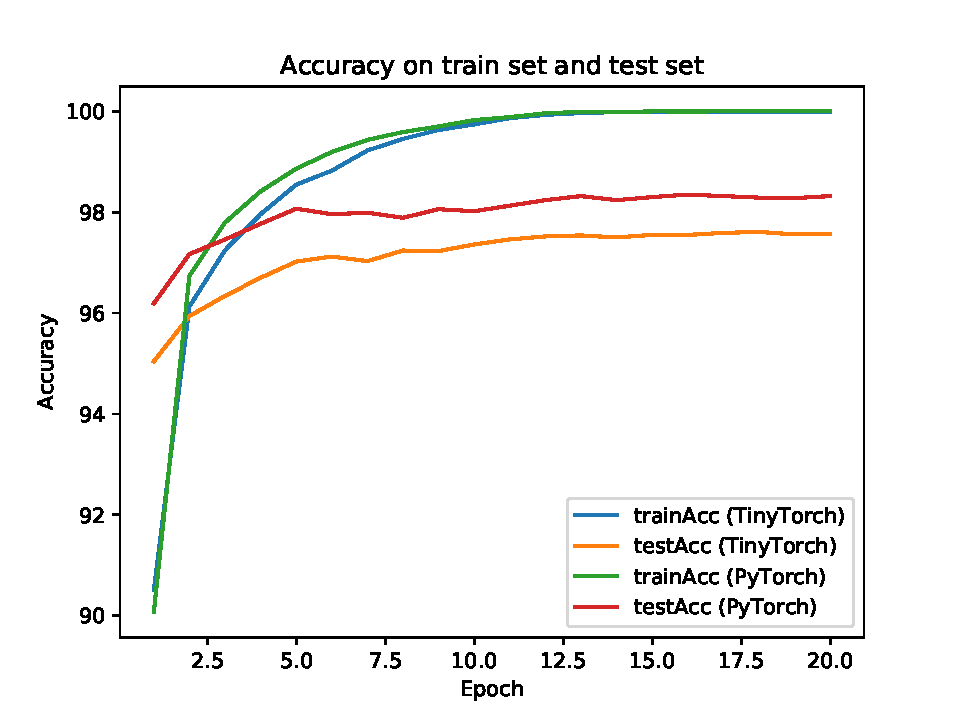
\includegraphics[width=0.6\linewidth]{fig/acc.pdf}
\caption{训练集及测试集精度}
\label{fig:acc}
\end{figure}

图\ref{fig:loss}展示了两个框架的训练损失,可以看到两者的训练损失都在快速下降,证明梯度下降的正确性。
\begin{figure}[H]
\centering
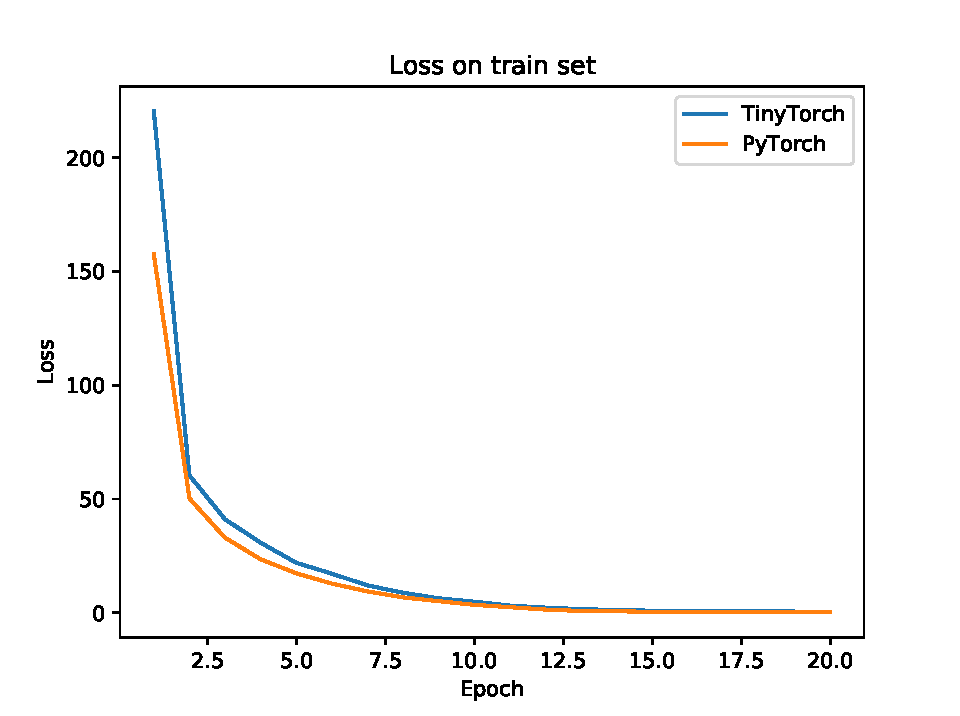
\includegraphics[width=0.6\linewidth]{fig/loss.pdf}
\caption{训练Loss}
\label{fig:loss}
\end{figure}

\section{总结}
本次实验自己搭建了TinyTorch的神经网络框架,虽然只有大约200行代码,且没有将自动微分功能实现,但还是熟悉了深度学习框架的整体设计及搭建流程。
最终可以用自己写的框架搭建起三层神经网络,并且做出来的结果也与PyTorch近似,基本算是达成目标。
后续如果有时间的话,则尝试将内置的Tensor类替换掉,然后实现自己的AD系统,真正搞懂深度学习框架的内部构造,而不再将其当成一个黑箱使用。

\section{附录:理论推导}
\label{sec:theory}
设$\smp{\vx}{i}$代表第$i$个训练样本,$\layer{\vz}{l}$代表第$l$层的输出,$\layer{\va}{l}$代表激活后的输出。
有三层神经网络的前向传播
\[\begin{aligned}
    \layer{\vz}{1} &= \layer{W}{1}\smp{\vx}{i} + \layer{\vb}{1}\\
    \layer{\va}{1} &= h(\layer{\vz}{1})\\
    \layer{\vz}{2} &= \layer{W}{2}\layer{\va}{1} + \layer{\vb}{2}\\
    \layer{\va}{2} &= h(\layer{\vz}{2})\\
    \layer{\vz}{3} &= \layer{W}{3}\layer{\va}{2} + \layer{\vb}{3}\\
    \hat{\vy}^{(i)} &=\layer{\va}{3} = g(\layer{\vz}{3})
\end{aligned}\]
其中真实结果$\vy^{(i)}$为独热码(one-hot encoding)。

考虑损失函数(loss)为交叉熵
\[\mL(\hat{\vy},\vy)=-\vy^\T\ln\hat{\vy}^{(i)}\]
且激活函数$h(\cdot)$为ReLU函数,$g(\cdot)$为softmax函数。

接下来推导反向传播(backpropagation, BP)算法,利用链式法则求导数。
比如想得到隐含层的权重,则计算
\[\pd{\mL}{\layer{W}{3}}=\pd{\mL}{\layer{\va}{3}}\pd{\layer{\va}{3}}{\layer{\vz}{3}}\pd{\layer{\vz}{3}}{\layer{W}{3}}\]
注意上式并非良定,其中涉及到实值函数对向量求导,也涉及到向量对向量求导(雅可比矩阵),还有向量对矩阵求导。
\[\begin{aligned}
\pd{\mL}{\layer{\va}{3}}
&=\pd{}{\layer{\va}{3}}(-\vy^\T\ln\hat{\va}^{[3]}) \qquad\mbox{实数对向量求导}\\
&=-\frac{\vy}{\layer{\va}{3}} \qquad\mbox{逐元素相除}
\end{aligned}\]

设$\vu=\exp(\layer{\vz}{3})$为逐元素指数,分两步计算
\[\begin{aligned}
\pd{\layer{\va}{3}}{\vu}
&=\pd{}{\vu}\softmax(\layer{\vz}{3})\\
&=\pd{}{\vu}\frac{\exp(\layer{\vz}{3})}{\vone^\T\exp(\layer{\vz}{3})}\\
&=\pd{}{\vu}\frac{\vu}{\vone^\T\vu}\\
&=\vu\pd{(1/\vone^\T\vu)}{\vu^\T}+\frac{1}{\vone^\T\vu}\pd{\vu}{\vu} \qquad\mbox{乘法法则}\\
&=-\frac{1}{(\vone^\T\vu)^3}\vu\vone^\T+\frac{1}{\vone^\T\vu}I\\
\pd{\vu}{\layer{\vz}{3}}
&=\pd{\exp(\layer{\vz}{3})}{\layer{\vz}{3}}\\
&=\opdiag(\exp(\layer{\vz}{3}))\\
&=\opdiag(\vu)
\end{aligned}\]

由雅可比矩阵的链式法则
\[\begin{aligned}
\pd{\layer{\va}{3}}{\layer{\vz}{3}}
&=\pd{\layer{\va}{3}}{\vu}\pd{\vu}{\layer{\vz}{3}}\\
&=\lrp{-\frac{1}{(\vone^\T\vu)^3}\vu\vone^\T+\frac{1}{\vone^\T\vu}I}\opdiag(\vu)\\
&=-\frac{1}{(\vone^\T\vu)^3}\vu\vu^\T+\frac{1}{\vone^\T\vu}\opdiag(\vu)\\
&=-\frac{\vu}{\vone^\T\vu}\lrp{\frac{\vu}{\vone^\T\vu}}^\T+\frac{1}{\vone^\T\vu}\opdiag(\vu)\\
&=-\layer{\va}{3}\layer{\va}{3}^\T+\opdiag(\layer{\va}{3})
\end{aligned}\]

进而
\[\begin{aligned}
\pd{\mL}{\layer{\vz}{3}}
&:=\layer{\delta}{3} \qquad\mbox{损失函数对未激活前$\vz$的导数}\\
&=\lrp{\pd{\layer{\va}{3}}{\layer{\vz}{3}}}^\T\pd{\mL}{\layer{\va}{3}}\\
&=-\lrp{-\layer{\va}{3}\layer{\va}{3}^\T+\opdiag(\layer{\va}{3})}^\T\lrp{\frac{\vy}{\layer{\va}{3}}}\\
&=\layer{\va}{3}\lrp{\layer{\va}{3}^\T\frac{\vy}{\layer{\va}{3}}}-\opdiag(\layer{\va}{3})\lrp{\frac{\vy}{\layer{\va}{3}}}\\
&=\layer{\va}{3}\vone^\T\vy-\vy\\
&=\layer{\va}{3}-\vy \qquad\mbox{独热码满足$\vone^\T\vy=1$}
\end{aligned}\]

之后可计算
\[\begin{array}{lll}
\pd{\mL}{\layer{W}{3}}&=\pd{\mL}{\layer{\vz}{3}}\pd{\layer{\vz}{3}}{\layer{W}{3}}
&=\layer{\delta}{3}\layer{\va}{2}^\T \qquad\mbox{线性变换求导法则}\\
\pd{\mL}{\layer{b}{3}}&=\pd{\mL}{\layer{\vz}{3}}\pd{\layer{\vz}{3}}{\layer{b}{3}}
&=\layer{\delta}{3}
\end{array}\]

再往前推一层
\[\begin{aligned}
\pd{\mL}{\layer{\va}{2}}
&=\layer{W}{3}^\T\layer{\delta}{3}\\
\pd{\mL}{\layer{\vz}{2}}
&:=\layer{\delta}{2}\\
&=\pd{\mL}{\layer{\va}{2}}\pd{\layer{\va}{2}}{\layer{\vz}{2}}\\
&=\pd{\mL}{\layer{\va}{2}}\odot h'(\layer{\vz}{2})\\
&=\lrp{\layer{W}{3}^\T\layer{\delta}{3}}\odot h(\layer{\vz}{2})\odot (\vone-h(\layer{\vz}{2}))\\
\pd{\mL}{\layer{W}{2}}&=\layer{\delta}{2}\vx^\T\\
\pd{\mL}{\layer{\vb}{2}}&=\layer{\delta}{2}\\
\pd{\mL}{\vx}&=\layer{W}{2}^\T\layer{\delta}{2}
\end{aligned}\]

总结来说,对于第$n_l$层,\textcolor{red}{
\[\layer{\delta}{n_l}=-(\vy-\layer{\va}{n_l})\odot g'(\layer{\vz}{n_l})=\layer{\tilde{\delta}}{n_l}\odot g'(\layer{\vz}{n_l})\]
}
对于第$l=n_l-1,n_l-2,\ldots,1$层,
\textcolor{red}{
\[\layer{\delta}{l}=\lrp{\layer{W}{l+1}^\T\layer{\delta}{l+1}}\odot h'(\layer{\vz}{l})=\layer{\tilde{\delta}}{l}\odot h'(\layer{\vz}{l})\]
}
则有权重和偏置的梯度\textcolor{red}{
\[\begin{aligned}
\nabla_{\layer{W}{l}}\mL(W,b)&=\layer{\delta}{l}\layer{\va}{l-1}^\T\\
\nabla_{\layer{b}{l}}\mL(W,b)&=\layer{\delta}{l}
\end{aligned}\]
}

\section{参考资料}
\begin{itemize}
	\item UFLDL Tutorial, \href{http://ufldl.stanford.edu/tutorial/supervised/MultiLayerNeuralNetworks/}{Multi-Layer Neural Network}
	\item Andrew Ng, Kian Katanforoosh, Anand Avati, \href{http://cs229.stanford.edu/notes2019fall/cs229-notes-deep_learning.pdf}{\emph{Stanford CS 229 Lecture Notes: Deep Learning}}
    \item Andrew Ng, Kian Katanforoosh, \href{http://cs229.stanford.edu/notes/cs229-notes-backprop.pdf}{\emph{Stanford CS 229 Lecture Notes: Backpropagation}}
    \item Kaare Brandt Petersen, Michael Syskind Pedersen, \href{https://www.math.uwaterloo.ca/~hwolkowi/matrixcookbook.pdf}{\emph{Matrix Cookbook}}
    \item \href{https://zhuanlan.zhihu.com/p/24709748}{矩阵求导术} - 长躯鬼侠的文章 - 知乎
    \item Daiwk,\href{https://daiwk.github.io/assets/matrix+vector+derivatives+for+machine+learning.pdf}{机器学习中的矩阵、向量求导}
	\item Guibo Wang, \href{https://borgwang.github.io/dl/2019/08/18/tinynn.html}{\emph{Build a Deep Learning Framework From Scratch}}
	\item Tianqi Chen, \href{https://dlsys.cs.washington.edu/}{UW CSE 599G1: Deep Learning System Course} - \href{https://github.com/dlsys-course/tinyflow}{TinyFlow}
\end{itemize}

\end{document}
% 请提交一份简短的实验报告,说明神经网络的实现过程以及模型在数据集上的表现。代码应有适量注释,并与报告一起提交。
% 说明:
% (1) 需要设计部分网络的结构,比如两层隐含层的神经元数,激活函数等;
% (2) 全连接层的参数初始化无需自己实现, 可直接调用函数;
% (3) 对类的设计没有具体要求, 在代码注释或报告中简要说明即可;